\begin{frame}
\frametitle{Regression of SHAP subgroups vs. hospital thrombolysis}

\begin{center}
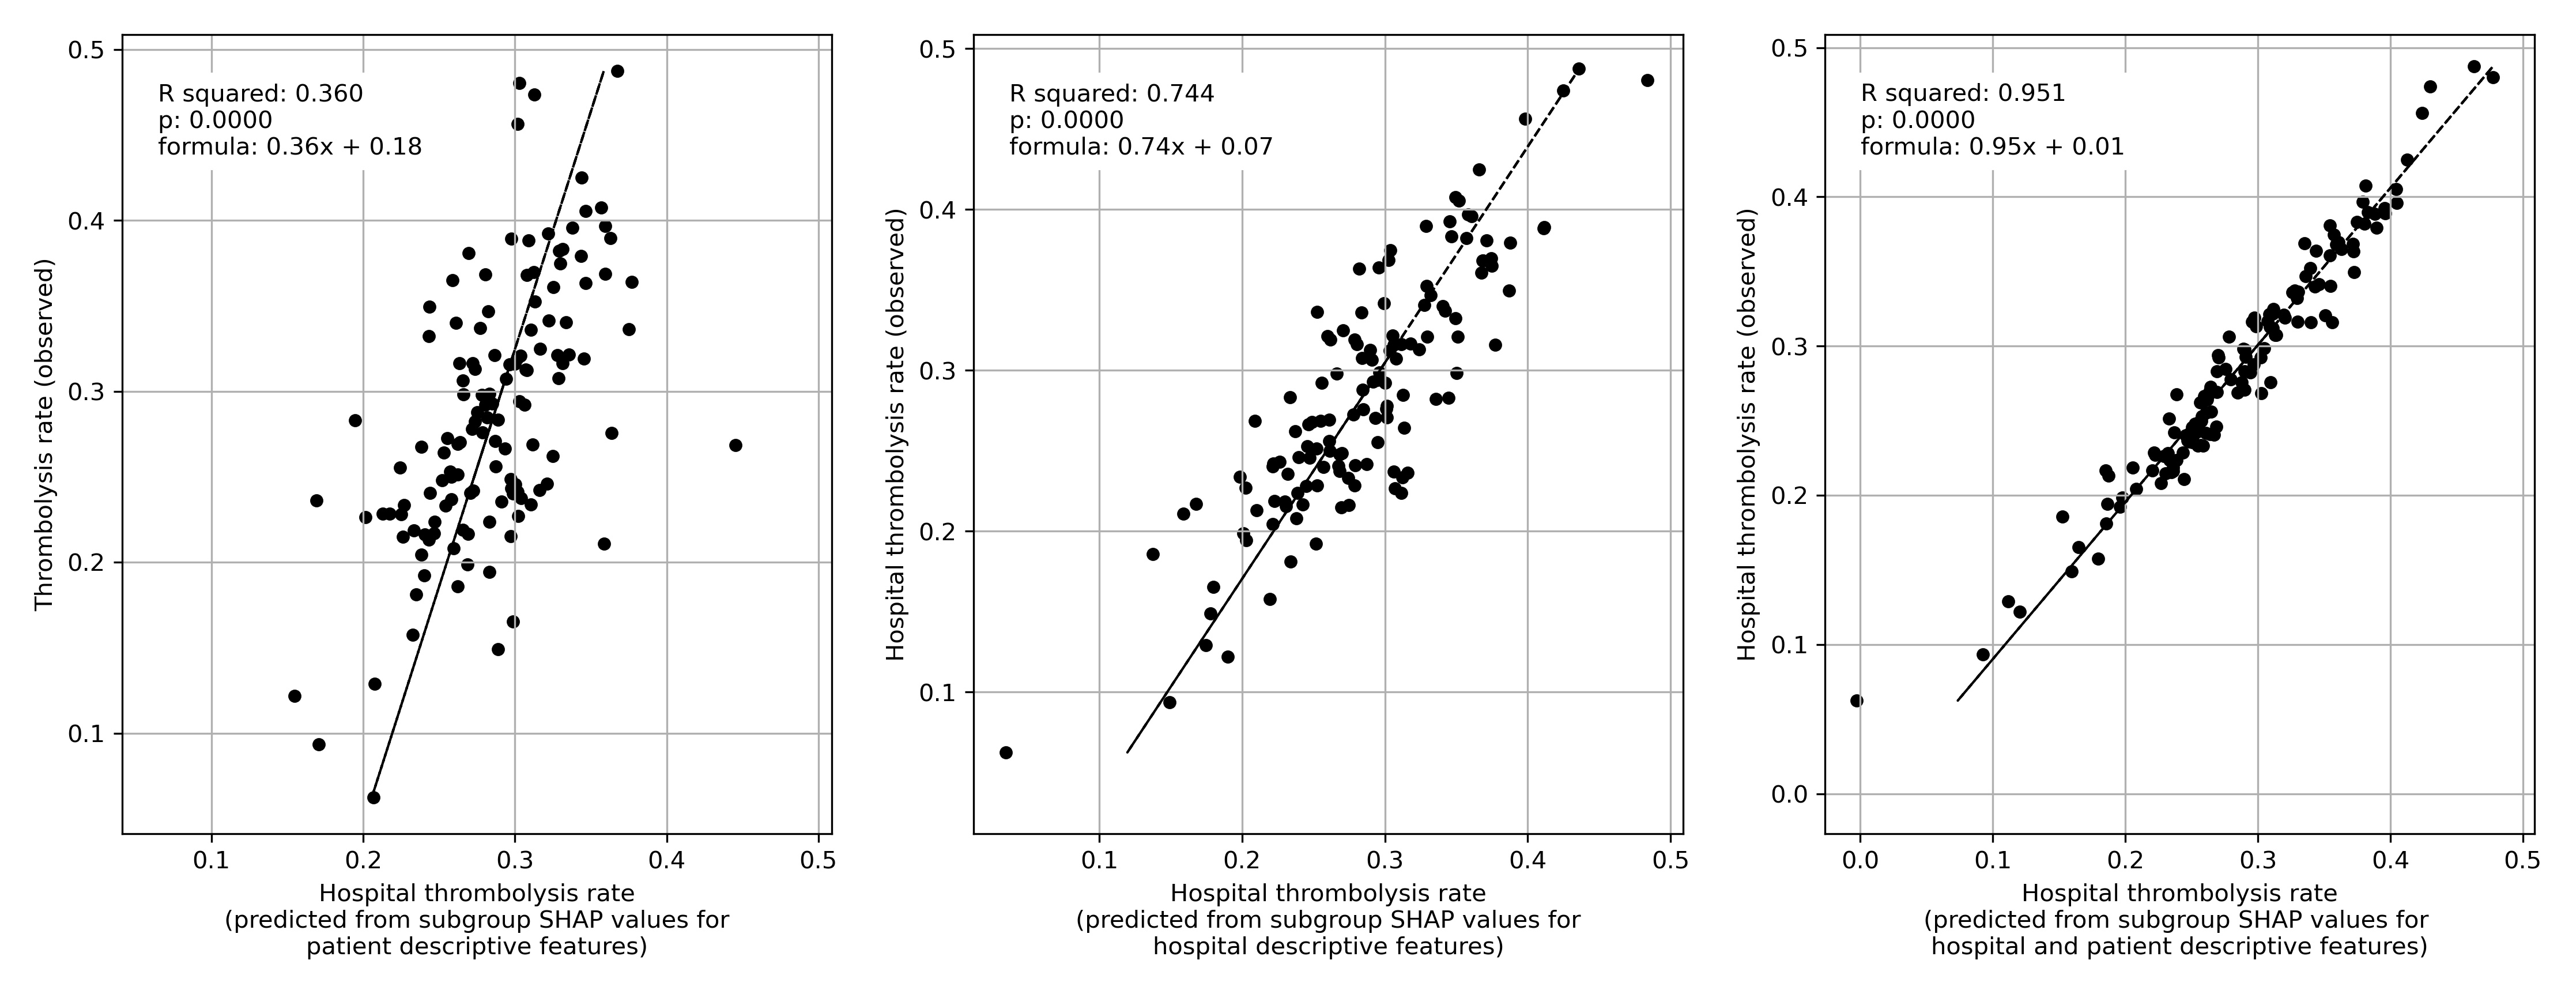
\includegraphics[width=0.95\textwidth]{./images/03e_xgb_10_features_multiple_regression_patient_hosptia_mean.jpg}
\end{center}

\scriptsize
\begin{itemize}
    \item Patient features (mean SHAP for each feature) alone explain 36\% of the variance in hospital thrombolysis use.
    \item Hospital features (mean SHAP for hospital ID and arrival-to-scan time) alone explains 74\% of the variance in hospital thrombolysis use. Hospital ID alone explains 58\% of the variance and arrival-to-scan time explains 23\% of the variance.
    \item Together, patient and hospital features explain 95\% of the variance in hospital thrombolysis use.
    \item Note: The sum of the patient-alone and hospital-one features = 110\%, suggesting we have a small amount of shared information between those groups.
\end{itemize}
 
\end{frame}